%% Based on  LaTeX template for ICML 2017 - example_paper.tex at 
%%  https://2017.icml.cc/Conferences/2017/StyleAuthorInstructions

\documentclass{article}
\usepackage[T1]{fontenc}
\usepackage{amssymb,amsmath}
\usepackage{txfonts}
\usepackage{microtype}
\usepackage{xspace}
\xspaceaddexceptions{\%}

% Lists with less spacoing between items
\usepackage{paralist}

% For figures
\usepackage{graphicx}
\usepackage{subfig} 

% For citations
\usepackage{natbib}

% For algorithms
\usepackage{algorithm}
\usepackage{algorithmic}

% the hyperref package is used to produce hyperlinks in the
% resulting PDF.  If this breaks your system, please commend out the
% following usepackage line and replace \usepackage{mlp2017} with
% \usepackage[nohyperref]{mlp2017} below.
\usepackage[hyphens]{url}
\urlstyle{same}
\usepackage{hyperref}

% Packages hyperref and algorithmic misbehave sometimes.  We can fix
% this with the following command.
\newcommand{\theHalgorithm}{\arabic{algorithm}}


% Set up MLP coursework style (based on ICML style)
\usepackage{mlp2018}
\mlptitlerunning{MLP Coursework 3 -- Interim Report (\groupNumber)}
\bibliographystyle{icml2017}


\DeclareMathOperator{\softmax}{softmax}
\DeclareMathOperator{\sigmoid}{sigmoid}
\DeclareMathOperator{\sgn}{sgn}
\DeclareMathOperator{\relu}{relu}
\DeclareMathOperator{\lrelu}{lrelu}
\DeclareMathOperator{\elu}{elu}
\DeclareMathOperator{\selu}{selu}
\DeclareMathOperator{\maxout}{maxout}







\DeclareMathOperator*{\argmax}{arg\,max}
\DeclareMathOperator*{\argmin}{arg\,min}
\DeclareMathOperator{\sg}{sg}
\DeclareMathOperator{\VQ}{VQ}

%% You probably do not need to change anything above this comment

\def\projectTitle{Improving End-to-End Voice Conversion using Discrete Latent Representations and Learnable Reconstruction Loss}
\def\groupNumber{G086}
\def\studentNumbers{s1873447, s1308389, s1837038}

\begin{document} 

\twocolumn[
\mlptitle{\projectTitle: Interim Report}

\centerline{\groupNumber\ (\studentNumbers)}

\vskip 7mm
]

\begin{abstract} 
Voice Conversion (VC) is widely desirable across many industries and applications, including speaker anonymization, film dubbing, gaming, and voice restoration for people who have lost their ability to speak. 
This work presents an end-to-end voice conversion method for unaligned corpora datasets.
Our model combines techniques from previous approaches, namely, 
a Variational Autoencoder with a discrete latent space due to a discrete latent interpretation of speech data (phonemes), 
GAN framework to make use of an adversarial loss for improving the clarity and voice style of the produced speech,
and a learned similarity metric to reduce artifacts in the output and improve intelligibility. 
Our model evaluation uses a architecture similar to WaveNet and will be trained on the Voice Cloning Toolkit
(VCTK) dataset and compared with two baseline approaches, VQ-VAE and VAW-GAN that have already been aplied to VC.

\end{abstract} 

\begin{figure*}[tb]
\vskip 5mm
\begin{center}
\centerline{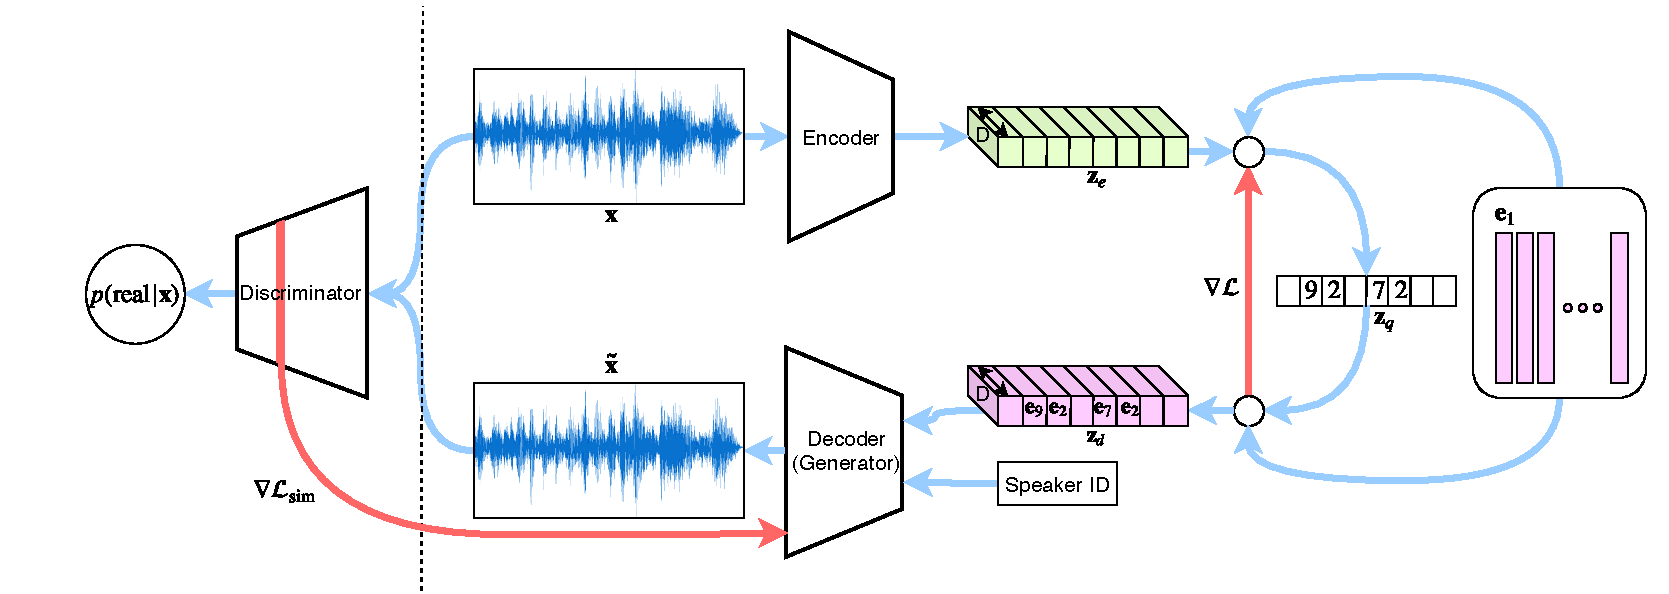
\includegraphics[width=0.95\textwidth]{report/figures/model.pdf}}
\caption{Architecture was mainly based on VQ-VAE with an addition of GAN and learnable similarity metric $\nabla \mathcal{L}_{\text{sim}}$. On the left we show the standard VQ-VAE architecture for VC. The embedding dictionary of the far-left is used both when producing the discrete latents $\mathbf{z}_q$ and mapping them back to vectors $\mathbf{z}_d$ for an input to the generator. The generator receives a one-hot encoded speaker identity, therefore the encoder can filter out the speaker-dependent features and only pertain the linguistic content. The red arrows also show how the gradient bypasses the discrete representations $\mathbf{z}_q$ and how similarity loss is used to improve the generator.
On the right, we also see the discriminator model, which takes both real data samples $\mathbf{x}$ and reconstructions from the generator $\mathbf{\tilde x}$ in order to improve the style of the generated content output.}
\label{fig:model-architecture}
\end{center}
\vskip -5mm
\end{figure*} 

\section{Introduction}
\label{sec:intro}
% This document provides a template for the MLP coursework 3 interim report.  This template structures the report into sections, which you may use,or you can structure it differently if you wish.  If you want to use subsections within a section that is fine. In this template the text in each section will include a very brief outline of what you should include in each section, along with some practical LaTeX examples (for example figures, tables, algorithms).  Your document should be no longer than \textbf{five pages},  with an additional page (or more!) allowed for references.

% You should give a broad introduction to the project, including citations to related work. Your aim here is to explain why the project is addressing an interesting topic, and how it relates to things that have been done in the area.

% You should make clear what are the aims and objectives of the project, what are the research questions being addressed.  Be precise. In this section you should make clear what the project's contribution is: how is it different to what is already done. 

% The interim report should state the objectives of the project, which are related to the research questions. What experiments do you plan to carry out? You can differentiate between core objectives, and optional objectives you hope to achieve if things go well. The conclusions in your final report should relate to these objectives.

% Use bibtex to organise your references -- in this case the references are in the file \verb+example-refs.bib+.  Here is a an example reference \citep{VandenOord2017}.  

The human voice conveys a multitude of non- or para-linguistic information about a speaker's identity, such as their age, gender, where they come from, or even their physical appearance~\citep{Kreiman2011}. Voice conversion (VC) is a speech processing field aiming to develop tools for transforming a person's (or a speech-synthesis system) speech to another target person's voice, without changing the linguistic content~\citep{Abe1990}. Applications include customised text-to-speech systems, speech-to-speech translation, film dubbing, speaker anonymisation, voice avatars in games, or speech-generating devices for people with speech impairments that aim to recreate the voices of their owners. Such systems are either trained on \textit{parallel} data, where source and target speakers utter the same sentences, or \textit{non-parallel} data where the sentences differ. Traditionally, approaches to parallel VC use time-frame alignment to generate labelled training data, while non-parallel VC may be approached with clustering methods to produce pseudo-parallel data or by using a conversion function that was learned from parallel data~\citep{Lorenzo2018}. More recently, however, VC has been approached as an unsupervised learning problem, where generative models can be trained end-to-end and do not require parallel data or clustering of source and target speakers utterances to perform VC. 

Generative modelling has recently made substantial advances in various domains, particularly images~\citep{Karras2018}, audio~\citep{Oord2016} or video~\citep{Vondrick2016}. While there are a number of different approaches to generative modelling, two frequently used methods are variational autoencoders (VAE)~\citep{Kingma2013} and generative adversarial networks (GANs) ~\citep{Goodfellow2014}.
GANs are an example of implicit latent variable models, where the functional form of the latent space can be arbitrarily complex, and is usually trained to match an unknown distribution of some dataset.
On the other hand, VAEs are an example of prescribed latent variable models, where assumptions about the latent density shape and noise are necessary. VAEs are trained to learn a low-dimensional latent representation of its inputs through a bottle-neck layer, minimising the reconstruction loss of the input data.
VC can be split into two models, speech encoder and speech synthesizer, where both of them can be treated as density learning problems. The task of the speech encoder is to find a compact and accurate representation of the linguistic content, and the task of the speech synthesizer is to generate speech that closely resembles the voice of the target speaker.

While latent variables are usually represented in a continuous space, many phenomena, such as phonemes, are better described in a discrete space, as argued e.g.  by~\cite{VandenOord2017}. Including discrete layers into a neural network, however, is not straight-forward, as no gradient can be computed directly. Vector-quantised variational autoencoders (VQ-VAE)~\cite{VandenOord2017} provide an extension to VAE by incorporating vector quantisation to obtain discrete latent variables. Evaluations show promising performance on image and video generation as well as voice conversion tasks~\cite{VandenOord2017}. %Furthermore, the authors were able to show that the discrete latent variables closely mapped to phonemes. 

Previous research has aimed to combine the strengths of VAE with those of GAN, in models such as VAE-GAN~\cite{Larsen2015} or AAE~\cite{Makhzani2015}, where a GAN can be used to provide a learned similarity metric for the VAE reconstruction loss. This aims to overcome the problem of element-wise metrics, which may not correspond to human judgements, as humans rather perceive higher-level features, rather than pixel-wise attributes ~\citep{Larsen2015}. 

As an optional objective for the present study, we investigate modifying the GAN framework to improve training performance. Regular GANs are known to suffer from training instability, and hence can be difficult to train. Wasserstein GAN (W-GAN) provide a modification of GAN, where the \textit{disciminator} is replaced with a \textit{critic} ~\citep{Arjovsky2017}. \cite{Hsu2017} have demonstrated the use of a Wasserstein generative adversarial network (VAW-GAN) to perform a VC task on non-parallel data, which outperformed a simple VAE. 

In the present work, we aim to combine recent developments in unsupervised representation learning to perform end-to-end VC on non-parallel data. More specifically, we investigate whether VC performance can be improved by combining the discrete representation from VQ-VAE with a GAN to model the voice style of the output more accurately, and whether using feature-wise reconstruction loss can improve the quality of the contents. Additionally, we address the question whether W-GAN can provide advantages over regular GAN in this scenario, in terms of training stability. 

In Section~\ref{sec:methodology}, we outline our general methodology and describe VQ-VAE, adversarial loss, the idea behind a learned similarity metric, W-GAN as well as our final model. in Section~\ref{sec:related-work}, we provide an overview of existing research and our contribution to improve them. Our experimental design and the dataset are described in Section~\ref{sec:experiments}. 
Section~\ref{sec:plan} contains a brief outline of issues that we still need to make decisions on and possible risks for our project. 

%VQ-VAE with learned similarity metric

%VAW-GAN\cite{Hsu2017}

%Phonetics(what we mostly care about at the moment), prosody(), etc. 

%Discrete (many to one mapping of latent variables to phonemes) vs. continuous latent representations. 

\section{Methodology}
\label{sec:methodology}
% Explain clearly the technical methodology, the models and algorithms that are used.  Approaches that were covered in the lectures can be described briefly, but if you are using modifications to such approaches make sure these are clearly described.    Again use citations to the literature.

% If you present algorithms, you can use the \verb+algorithm+ and \verb+algorithmic+ environments to format pseudocode (for instance, Algorithm~\ref{alg:example}). These require the corresponding style files, \verb+algorithm.sty+ and \verb+algorithmic.sty+ which are supplied with this package. 

% \begin{algorithm}[ht]
% \begin{algorithmic}
%   \STATE {\bfseries Input:} data $x_i$, size $m$
%   \REPEAT
%   \STATE Initialize $noChange = true$.
%   \FOR{$i=1$ {\bfseries to} $m-1$}
%   \IF{$x_i > x_{i+1}$} 
%   \STATE Swap $x_i$ and $x_{i+1}$
%   \STATE $noChange = false$
%   \ENDIF
%   \ENDFOR
%   \UNTIL{$noChange$ is $true$}
% \end{algorithmic}
%   \caption{Bubble Sort}
%   \label{alg:example}
% \end{algorithm}
In unaligned corpora voice conversion task we have a dataset of recorded utterances from a set of speakers where the linguistic content of the recordings may not be matched.
% In such problems, VC techniques using recurrent encoder-decoder networks do not usually work well.
In this work, we assume that the spectral frames $\mathbf{x}$ of the recordings come from a true probability density, and that the densities for the source and target speakers are $p_s$ and $p_t$. The VC task is then to learn a conditional distribution $q_t$ on $\mathbf{x}_s \sim p_s$ such that $q_t \approx p_t$.
Moreover, reflecting on the traditional VC pipelines, we assume that speech can be encoded as a discrete low-dimensional code, namely a vector of phonemes. In the rest of this section we propose an end-to-end VC method takes advantage of this interpretation.


\subsection{VQ-VAE for learning discrete latents}
\label{sec:methodology:vq-vae}
Variational Autoencoders (VAE)~\cite{Kingma2013} are widely popular for their ability to learn unobserved low-dimensional latent distributions $p_z$ of observed high-dimensional data $p_x$. VAEs are two-part models consisting of: an \textit{encoder} $E$  that approximates the conditional distribution $p(\mathbf{z}|\mathbf{x})$ with a parameterised model, and \textit{decoder} that generates samples from the original distribution $p_x$ given samples from $\mathbf{z}$, namely $p(\mathbf{x}|\mathbf{z})$.
In our work, we will refer to the decoder as \textit{generator} $G$, since it is tasked to synthesise realistic data samples, as we will see in the next section.

The latent distributions in standard VAEs are typically diagonal-covariance Gaussian. 
However, in VC we prefer to filter out most of the speaker-related variance and noise, and focus only on the discrete linguistic content, i.e. phonemes, that preserves the most relevant information for the task. 
In order to take advantage of discrete speech interpretation we use Vector-Quantised VAE (VQ-VAE)~\citep{VandenOord2017} where a discrete embedding layer ($\VQ$) is inserted between the encoder and generator.
The embedding layer contains a dictionary of $K$ $D$-dimensional real-valued embedding vectors $\mathbf{e}_k$, where $k = 1..K$ and $K$ is the number of discrete values allowed by the dictionary.
The $\VQ$ layer takes the output from the encoder $\mathbf{z}_e = E({\mathbf{x}})$ and calculates the discrete latent value $z_q=k$ by a nearest neighbour look-up in the dictionary of embeddings, where $k$ is the index of the embedding vector $\mathbf{e}_k$ that minimises distance to $\mathbf{z}_e$:
\begin{equation}
    \label{eq:nearest-neighbour}
    z_q = k = \argmin_i || \mathbf{z}_e - \mathbf{e}_i ||_2
\end{equation}
Then the closest embedding vector $\mathbf{e}_k$ (the one that minimises the objective above) is passed down as input $\mathbf{z}_g = \mathbf{e}_k = \VQ(\mathbf{z}_e)$ to the generator network. For simplicity, the example above assumed that the input to the $\VQ$ layer $\mathbf{z}_e$ was a $D$-dimensional vector mapped to a single latent variable $z_q$. 
However, in general the output can be any tensor whose channel is $D$-dimensional, then the nearest-neighbour quantization described in Eq.~\ref{eq:nearest-neighbour} is applied to each element along the channel dimension.
In the VC task it will be a $Z \times D$ tensor, where $Z$ is the length of the down-sampled recording.
% (from paper) VQ layer can be viewed as a particular type of non-linearity.

\begin{figure}[tb]
\vskip 5mm
\begin{center}
\centerline{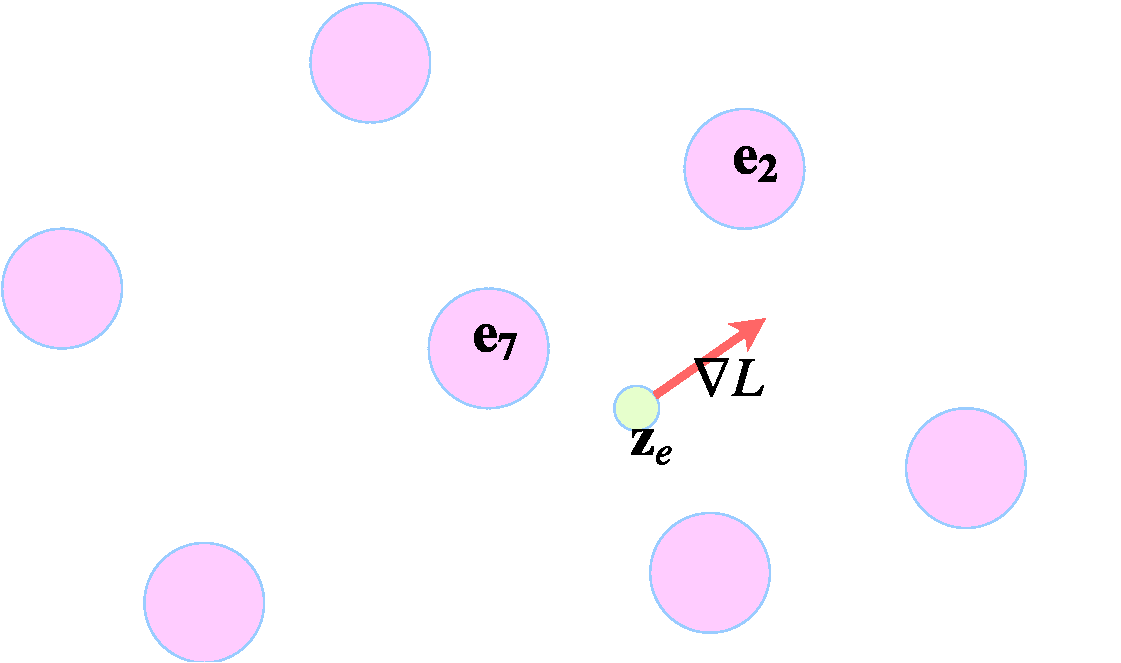
\includegraphics[width=0.8\columnwidth]{report/figures/embedding.pdf}}
\caption{The figure shows how the straight-through estimator gradient can help the encoder to produce samples from a different category in the next forward pass. I.e. if in the current run the vector $\mathbf{z}_e$ was assigned by nearest-neighbour distance to $\mathbf{e_7}$, then the straight-through gradient estimator can push the encoder output vector closer to $\mathbf{e}_2$ in the next forward run. This is a reasonable assumption, since the straight-through estimator guarantees the signs of the gradient to be correct \citep{Bengio2013}.}
\label{fig:vq-vae-embedding}
\end{center}
\vskip -5mm
\end{figure} 

Generally, training models with discrete layers is difficult since there is no gradient. However, since the gradient needs to propagate through only a single discrete layer, VQ-VAE can use a straight-through gradient estimator copying the gradients from the generator input $\mathbf{z}_g$ to encoder output $\mathbf{z}_e$ bypassing the $VQ$ layer. The signs of the straight-through gradient estimator are guaranteed to be correct when propagating through a single layer \citep{Bengio2013} and should contain useful information for training the outputs of the encoder as illustrated on the right side of the Figure~\ref{fig:vq-vae-embedding}.

The VQ-VAE loss function comprises of three terms -- reconstruction loss, vector quantisation (embedding training) objective, and commitment loss:
\begin{equation}
    \label{eq:vq-vae-rec-loss}
    \mathcal{L}_{\text{rec}} = \log(p(\mathbf{x}|E(\mathbf{x})))
\end{equation}
\begin{equation}
    \label{eq:vq-vae-vq-loss}
    \mathcal{L}_{\VQ} = ||\sg[E(\mathbf{x})] - \mathbf{e}||_2^2
\end{equation}
\begin{equation}
    \label{eq:vq-vae-commit-loss}
    \mathcal{L}_{\text{com}} = \beta||E(\mathbf{x}) - \sg[\mathbf{e}]||^2_2
\end{equation}
The reconstruction loss in Eq.~\ref{eq:vq-vae-rec-loss} optimises the encoder and generator model parameters to pertain the contents of the original input, however due to the straight-through gradient estimation the embedding vectors $\mathbf{e}$ of the $\VQ$ layer are not updated. 
In order to train the embedding vectors the vector quantisation objective in Eq.~\ref{eq:vq-vae-vq-loss} is added to directly trains the embedding vectors $\mathbf{e}$ to minimise the $l_2$ distance to the encoder output $\mathbf{z}_e$. 
Moreover, because the embedding space is dimensionless (it is not bound to any physical quantity) it can grow arbitrarily if the encoder does not train as fast as the embedding vectors. Therefore, the commitment loss in Eq.~\ref{eq:vq-vae-commit-loss} is added to constrain the growth of the embedding space. 
Finally, despite the term "variational" in its name, the loss does not contain a variational loss objective because the prior $p(\mathbf{z})$ is assumed uniform and the KL-divergence term simplifies to a constant $\log K$.

The $\sg(.)$ in Eq.~\ref{eq:vq-vae-vq-loss} and \ref{eq:vq-vae-commit-loss} is a stop-gradient operator defined as:
\begin{equation}
    \sg(\mathbf{x}) = 
    \begin{cases}
    \mathbf{x},  & \text{forward pass}\\
    \mathbf{0},  & \text{backward pass}
    \end{cases}
\end{equation}

Our implementation of the VQ layer in PyTorch will be published with the project code in a public repository as a pluggable layer for use in different network architectures.

\subsection{Improving the generator with adversarial loss}
\label{sec:methodology:adversarial-loss}
The output of VAEs in image and speech domains is typically blurry due to the element-wise $l_2$ reconstruction loss, which is equivalent to maximising the log-likelihood of data $p(\mathbf{x}|\mathbf{\hat x})$ and assuming it is Gaussian. However, real data such as images and speech are usually multimodal and therefore the Gaussianity assumption is too general. In particular, in VC task we would like the output of the VQ-VAE match the probability distribution of spectral frames of the target speaker.

Generative Adversarial Networks (GAN) \cite{Goodfellow2014} have become particularly popular due to their ability to train a generator that can synthesise samples from an arbitrarily complex and unknown distributions. 
The main components of a GAN are the \textit{generator} $G$, \textit{discriminator} $D$, and adversarial loss. 
The purpose of the generator is to learn a transformation from a prior "noise" distribution $p_z$ to the true data distribution $p_x$. 
The discriminator takes the output from the generator $\mathbf{\tilde x}$ and examples from the true dataset $\mathbf{x}$, and is tasked to output a single scalar corresponding to the probability that its input came from the real dataset rather than the output from the generator, which is considered a "fake" sample. The training objective called adversarial loss is described by the below equation:
\begin{equation}
    \mathcal{L}_{adv} = \log(D(\mathbf{x})) + \log(1-D(G(\mathbf{z}_g))),
\end{equation}
where in our work the latents $\mathbf{z}_g$ are the encoded and quantised versions of input, $\mathbf{z}_g = \VQ(E(\mathbf{x}))$.

In our work, the generator of the GAN is the same network as the decoder in VQ-VAE.
We employ GAN framework in order to train the generator(decoder) more directly to match the target distribution more accurately via adversarial loss.


\subsection{Improving the generator with learned similarity metric}
To loosen the Gaussianity assumption about the true dataset implied by element-wise loss we here consider an alternative reconstruction error. We first assume that the discriminator must learn a useful internal representation of the input data in order to distinguish real from fake samples. We then adapt learnable feature-wise reconstruction metric from \citet{Larsen2015} to replace the reconstruction error in Eq.~\ref{eq:vq-vae-rec-loss}.

The metric introduces a Gaussian observation model on the hidden representations of the discriminator:
\begin{equation}
    \label{eq:similarity-metric}
    p(D_l(\mathbf{x})|\mathbf{z}_g) = \mathcal{N}(D_l(\mathbf{x})|D_l(G(\mathbf{z}_g)), \mathbf{I}),
\end{equation}
where $D_l(\mathbf{x})$ is the hidden representation of input $\mathbf{x}$ in layer $l$ of the discriminator, and $\mathbf{z}_g$ is the input to the generator for input $\mathbf{x}$. 
The reconstruction term in Eq.~\ref{eq:vq-vae-rec-loss} is then replaced with the feature-wise similarity error shown in Eq.~\ref{eq:similarity-error}, thus resulting in content-wise better reconstructions.
\begin{equation}
    \label{eq:similarity-error}
    \mathcal{L}_{\text{sim}} = - \mathbb{E}_{q(\mathbf{z_g}|\mathbf{x})}[\log p(D_l(\mathbf{x})|\mathbf{z}_g)]
\end{equation}
It is important that the error signal from Eq.~\ref{eq:similarity-metric} is only used to train the VQ-VAE but not the discriminator as this would otherwise collapse the gradients to 0 \citep{Larsen2015}.


\subsection{W-GAN}
\label{sec:methodology:w-gan}
Previous work has explored the instability that is typically observed when training GANs~\cite{arjovsky2017towards}.
Their conclusion was that this instability comes from the training procedure's ability to result in degenerate states where both networks are unable to learn. One example of this is in the case of a perfect discriminator network which causes the gradient to collapse to zero.

Wasserstein GANs (W-GANs)~\cite{Arjovsky2017} provide an alternate method of training these networks in a more stable manner. This is achieved by replacing the Jensen-Shannon divergence metric of standard GANs with the Earth-Mover (EM) distance (also referred to as the Wasserstein-1 distance). For this to work, the discriminator network is replaced with a critic network where the difference is that it outputs a scalar value instead of probability. These changes cause the gradient updates to become much more stable because the EM distance has a smoother gradient and both the generator and critic networks can be trained until optimality.

\subsection{Final model}
Our final model stems directly from a combination of methods introduced in the previous sections and is presented in Figure~\ref{fig:model-architecture}. The model leverages discrete latent variable interpretation of speech data through vector quantisation, employs an adversarial loss to improve the realistic style of synthesised reconstructions, and uses a learned similarity metric to pertain the linguistic contents of the input data in the generated outputs. The complete loss function is as follows:
\begin{equation}
    \mathcal{L} = \mathcal{L}_{\text{sim}} + \mathcal{L}_{\VQ} + \mathcal{L}_{\text{com}} + \mathcal{L}_{\text{adv}}
\end{equation}

We note that the speaker identity code is provided directly to the generator as shown in Figure~\ref{fig:model-architecture}, thus the encoder is allowed to filter out speaker-dependent features in spite of keeping only the linguistic content. Voice conversion can then be achieved by providing the target speaker identity code to the generator and latent code $\mathbf{z}_g$ from the source speaker.

% To create figure (just made a start so far - the tool seems quite cool): https://drive.google.com/file/d/1AvEt7xVth1SRBc0uVrzy1jWwvI600KeH/view?usp=sharing

\section{Related work}
\label{sec:related-work}
In this work we have presented a new model for end-to-end voice conversion based on a combination of several popular methods and is described in the previous section.

Earlier end-to-end VC methods used a traditional VAE with isotropic Gaussian assumption on the latent space \citep{Hsu2016}, and found successful results. A further study (VAW-GAN) \citep{Hsu2017} has found that introducing an adversarial loss can enhance variability in the frequency axis, and hence results in improved voice clarity. 

The paper on VQ-VAE \citep{VandenOord2017} has also reported promising results for voice conversion task. Most significantly, the authors have shown that VQ-VAE can learn to classify phonemes in its latent layer with about 47\% accuracy (random classification would have been about 7\%) in a completely unsupervised manner.

Our work merges these ideas and evaluates their benefits in the next section. In addition, we also adapted a learnable feature-wise similarity metric method from image processing \citep{Larsen2015}, replacing the element-wise metric in VAE reconstruction loss, to improve the intelligibility of the synthesised speech.

\section{Experiments}
\label{sec:experiments}
% The interim report should include some experimental results.  In most cases these will be baseline experiments.  Baseline experiments refer to experiments conducted using well-understood approaches against which you can compare later results.  For example if you were exploring a new data set, the baselines might include linear networks and deep neural networks with different numbers of hidden layers;  if you were exploring a different approach to regularisation, then the baselines would include no regularisation, and conventional techniques such as L1, L2, and dropout.  You can include the results of any further experiments in your interim report.

% Present the experimental results clearly and concisely.  Usually a result is in comparison or contrast to a result from another approach please make sure that these comparisons/contrasts are clearly presented.  You can facilitate comparisons either using graphs with multiple curves or (if appropriate, e.g. for accuracies) a results table. You need to avoid having too many figures, poorly labelled graphs, and graphs which should be comparable but which use different axis scales. A good presentation will enable the reader to compare trends in the same graph -- each graph should summarise the results relating to a particular research (sub)question.

% There is no need to include code or specific details about the compute environment.

% As before, your experimental sections should include graphs (for instance, figure~\ref{fig:sample-graph}) and/or tables (for instance, table~\ref{tab:sample-table})\footnote{These examples were taken from the ICML template paper.}, using the \verb+figure+ and \verb+table+ environments, in which you use \verb+\includegraphics+ to include an image (pdf, png, or jpg formats).  Please export graphs as 
% \href{https://en.wikipedia.org/wiki/Vector_graphics}{vector graphics}
% rather than \href{https://en.wikipedia.org/wiki/Raster_graphics}{raster
% files} as this will make sure all detail in the plot is visible.
% Matplotlib supports saving high quality figures in a wide range of
% common image formats using the
% \href{http://matplotlib.org/api/pyplot_api.html\#matplotlib.pyplot.savefig}{\texttt{savefig}}
% function. \textbf{You should use \texttt{savefig} rather than copying
% the screen-resolution raster images outputted in the notebook.} An
% example of using \texttt{savefig} to save a figure as a PDF file (which
% can be included as graphics in a \LaTeX document is given in the coursework document.

% If you need a figure or table to stretch across two columns use the \verb+figure*+ or \verb+table*+ environment instead of the \verb+figure+ or \verb+table+ environment.  Use the \verb+subfigure+ environment if you want to include multiple graphics in a single figure.

% \begin{figure}[tb]
% \vskip 5mm
% \begin{center}
% \centerline{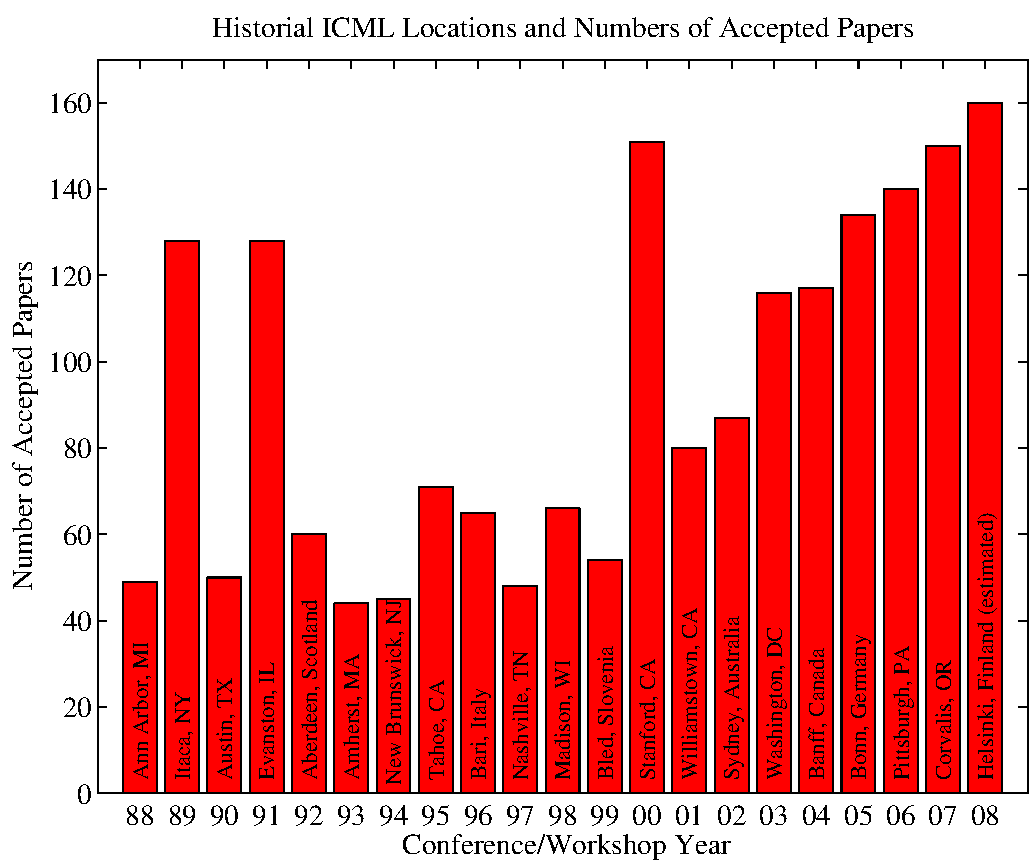
\includegraphics[width=\columnwidth]{icml_numpapers}}
% \caption{Historical locations and number of accepted papers for International
%   Machine Learning Conferences (ICML 1993 -- ICML 2008) and
%   International Workshops on Machine Learning (ML 1988 -- ML
%   1992). At the time this figure was produced, the number of
%   accepted papers for ICML 2008 was unknown and instead estimated.}
% \label{fig:sample-graph}
% \end{center}
% \vskip -5mm
% \end{figure} 

% \begin{table}[tb]
% \vskip 3mm
% \begin{center}
% \begin{small}
% \begin{sc}
% \begin{tabular}{lcccr}
% \hline
% \abovespace\belowspace
% Data set & Naive & Flexible & Better? \\
% \hline
% \abovespace
% Breast    & 95.9$\pm$ 0.2& 96.7$\pm$ 0.2& $\surd$ \\
% Cleveland & 83.3$\pm$ 0.6& 80.0$\pm$ 0.6& $\times$\\
% Glass2    & 61.9$\pm$ 1.4& 83.8$\pm$ 0.7& $\surd$ \\
% Credit    & 74.8$\pm$ 0.5& 78.3$\pm$ 0.6&         \\
% Horse     & 73.3$\pm$ 0.9& 69.7$\pm$ 1.0& $\times$\\
% Meta      & 67.1$\pm$ 0.6& 76.5$\pm$ 0.5& $\surd$ \\
% Pima      & 75.1$\pm$ 0.6& 73.9$\pm$ 0.5&         \\
% \belowspace
% Vehicle   & 44.9$\pm$ 0.6& 61.5$\pm$ 0.4& $\surd$ \\
% \hline
% \end{tabular}
% \end{sc}
% \end{small}
% \caption{Classification accuracies for naive Bayes and flexible 
% Bayes on various data sets.}
% \label{tab:sample-table}
% \end{center}
% \vskip -3mm
% \end{table}

% In order to evaluate the performance of our proposed model we will train two additional models, the VQ-VAE and VAE-GAN, on the same dataset which will serve as baselines.
In the experiments we want to evaluate the benefits of the introducing a combination of methods to unaligned voice conversion task. We therefore set two baseline experiments using a simple VQ-VAE and VAW-GAN that have already shown to provide successful results.

Next, we will combine VQ-VAE with an adversarial loss and observe whether the converted speech is clearer an more intelligible, and whether the use of vector quantised latents improves the contents over VAW-GAN.
And finally, we replace the element-wise reconstruction loss of VAE with a learnable feature-wise loss and observe whether it preserves the content of the speech better.

In the experiments we will use a simplified WaveNet architecture \cite{Oord2016} consisting of dilated convolutional layers. The encoder and generator networks will not use fully-connected layers and therefore should be able to process inputs of various length. Further details about the architecture will be added in the final report once they are finally decided.

\subsection{Dataset} 
\label{sec:experiments:dataset}
%Clearly describe the data set and task you will be exploring.  If the data requires any preprocessing, then explain this.  The description should be in enough detail such that your work would be reproducible by another group.  Describe how you will evaluate the task (for example, classification accuracy).  Use citations where appropriate.

To tackle the problem of VC, the Voice Cloning Toolkit (VCTK) dataset~\cite{yamagishi_english_2012} was chosen which includes speech from 109 different speakers of English. For each speaker there is audio data for approximately 400 sentences on average, taken from a number of different sources including a newspaper. The data is non-parallel meaning that the speech is not necessarily aligned and the spoken content may not even be the same. Each spoken sentence is given as a separate file in Waveform Audio File Format (WAVE) which allows it to be easily read by available tools and used directly by our model. Since our model is trained end to end, the input is the raw waveform and no pre-processing stages are required.

% \section{Interim conclusions}
% \label{sec:concl}
% What have you learned so far?  Do the experiments indicate that the project is feasible?  Do the experiments indicate that you should consider changes to your original plan?  Can you compare your results so far to what has been reported in the literature?

\section{Plan}
\label{sec:plan}
% Based on what you have done so far, present a plan for the rest of the project.  Are there any changes to the objectives?  What are the risks?  Do you need a backup plan?

We have so far implemented the VQ layer only. The next steps are to implement the baseline models that were outlined in Section~\ref{sec:experiments} to see if we can achieve comparable performance to previous work and have some results for relative comparison. While these models for VC are often evaluated qualitatively by human raters, we aim to also provide some quantitative measure of performance although this is yet to be determined. 

Through our experiments we aim to test the relative performance after making incremental changes from the baselines to the final model. If the addition of discrete layer to our model does not improve the performance of our model, we can still switch to using a continuous representation as the distance metric is still a new addition.

\bibliography{refs}

\end{document} 

